\documentclass[UTF8]{article}
\usepackage{graphicx}
\usepackage{subfigure}
\usepackage{amsmath}
\usepackage{makecell}
\usepackage[utf8]{inputenc}
\usepackage[space]{ctex} %中文包
\usepackage{listings} %放代码
\usepackage{xcolor} %代码着色宏包
\usepackage{CJK} %显示中文宏包
\usepackage{float}
\usepackage{makecell}
\usepackage{diagbox}
\usepackage{bm}
\usepackage{ulem} 
\usepackage{amssymb}
\usepackage{soul}
\usepackage{color}
\usepackage{geometry}
\usepackage{fancybox} %花里胡哨的盒子
\usepackage{xhfill} %填充包, 可画分割线 https://www.latexstudio.net/archives/8245
\usepackage{multicol} %多栏包
\usepackage{enumerate} %可以方便地自定义枚举标题
\usepackage{multirow} %表格中多行单元格合并
\usepackage{wasysym} %可以使用wasysym里的一堆奇奇怪怪的符号
\usepackage{tikz}
\usetikzlibrary{shadows} % 阴影支持
\usepackage{pgfplotstable}% recommended:%\usepackage{booktabs}%\usepackage{array}%\usepackage{colortbl}
\usepackage{enumitem}
\AddEnumerateCounter{\chinese}{\chinese}{}

\geometry{left = 1cm, right = 1cm, top=1cm, bottom=2cm}

\definecolor{mygreen}{rgb}{0,0.6,0}
\definecolor{mygray}{rgb}{0.5,0.5,0.5}
\definecolor{mymauve}{rgb}{0.58,0,0.82}
\lstset{
	backgroundcolor=\color{white}, 
	%\tiny < \scriptsize < \footnotesize < \small < \normalsize < \large < \Large < \LARGE < \huge < \Huge
	basicstyle = \footnotesize,       
	breakatwhitespace = false,        
	breaklines = true,                 
	captionpos = b,                    
	commentstyle = \color{mygreen}\bfseries,
	extendedchars = false,
	frame = shadowbox, 
	framerule=0.5pt,
	keepspaces=true,
	keywordstyle=\color{blue}\bfseries, % keyword style
	language = C++,                     % the language of code
	otherkeywords={string}, 
	numbers=left, 
	numbersep=5pt,
	numberstyle=\tiny\color{mygray},
	rulecolor=\color{black},         
	showspaces=false,  
	showstringspaces=false, 
	showtabs=false,    
	stepnumber=1,         
	stringstyle=\color{mymauve},        % string literal style
	tabsize=4,          
	title=\lstname           
}

%\sum\nolimits_{j=1}^{M}   上下标位于求和符号的水平右端,
%\sum\limits_{j=1}^{M}   上下标位于求和符号的上下处,
%\sum_{j=1}^{M}  对上下标位置没有设定,会随公式所处环境自动调整。

%%%%%%%%%%%%%画图包%%%%%%%%%%%%%
\usepackage{tikz}
%%%%%%%%%%%%%好看的矩形%%%%%%%%%%%%%
\tikzset{
  rect1/.style = {
    shape = rectangle,% 指定样式
    minimum height=2cm,% 最小高度
    minimum width=4cm,% 最小宽度
    align = center,% 文字居中
    drop shadow,% 阴影
  }
}
%%%%%%%%%%%%%画图背景包%%%%%%%%%%%%%
\usetikzlibrary{backgrounds}

%%%%%%%%%%%%%在tikz中画一个顶点%%%%%%%%%%%%%
%%%%%%%%%%%%%#1:node名称%%%%%%%%%%%%%
%%%%%%%%%%%%%#2:位置%%%%%%%%%%%%%
%%%%%%%%%%%%%#3:标签%%%%%%%%%%%%%
\newcommand{\newVertex}[3]{\node[circle, draw=black, line width=1pt, scale=0.8] (#1) at #2{#3}}
%%%%%%%%%%%%%在tikz中画一条边%%%%%%%%%%%%%
\newcommand{\newEdge}[2]{\draw [black,very thick](#1)--(#2)}
%%%%%%%%%%%%%在tikz中放一个标签%%%%%%%%%%%%%
%%%%%%%%%%%%%#1:名称%%%%%%%%%%%%%
%%%%%%%%%%%%%#2:位置%%%%%%%%%%%%%
%%%%%%%%%%%%%#3:标签内容%%%%%%%%%%%%%
\newcommand{\newLabel}[3]{\node[line width=1pt] (#1) at #2{#3}}

%%%%%%%%%%%%%强制跳过一行%%%%%%%%%%%%%
\newcommand{\jumpLine} {\hspace*{\fill} \par}
%%%%%%%%%%%%%关键点指令,可用itemise替代%%%%%%%%%%%%%
\newcommand{\average}[1]{\left\langle #1\right\rangle }
%%%%%%%%%%%%%表格内嵌套表格%%%%%%%%%%%%%
\newcommand{\keypoint}[2]{$\bullet$\textbf{#1}\quad#2\par}
%%%%%%%%%%%%%<T>平均值表示%%%%%%%%%%%%%
\newcommand{\tabincell}[2]{\begin{tabular}{@{}#1@{}}#2\end{tabular}}%放在导言区
%%%%%%%%%%%%%大黑点item头%%%%%%%%%%%%%
\newcommand{\itemblt}{\item[$\bullet$]}
%%%%%%%%%%%%%大圈item头%%%%%%%%%%%%%
\newcommand{\itemc}{\item[$\circ$]}
%%%%%%%%%%%%%大星星item头%%%%%%%%%%%%%
\newcommand{\itembs}{\item[$\bigstar$]}
%%%%%%%%%%%%%右▷item头%%%%%%%%%%%%%
\newcommand{\itemrhd}{\item[$\rhd$]}
%%%%%%%%%%%%%定义为%%%%%%%%%%%%%
\newcommand{\defas}{=_{df}}
%%%%%%%%%%%%%蕴含%%%%%%%%%%%%%
\newcommand{\imp}{\rightarrow}

%%%%%%%%%%%%%双线分割线%%%%%%%%%%%%%
\newcommand*{\doublerule}{\hrule width \hsize height 1pt \kern 0.5mm \hrule width \hsize height 2pt}
%%%%%%%%%%%%%双线中间可加东西的分割线%%%%%%%%%%%%%
\newcommand\doublerulefill{\leavevmode\leaders\vbox{\hrule width .1pt\kern1pt\hrule}\hfill\kern0pt }
%%%%%%%%%%%%%左大括号%%%%%%%%%%%%%
\newcommand{\leftbig}[1]{\left\{\begin{array}{l}#1\end{array}\right.}
%%%%%%%%%%%%%矩阵%%%%%%%%%%%%%
\newcommand{\mat}[2]{\left[\begin{array}{#1}#2\end{array}\right]}
%%%%%%%%%%%%%可换行圆角文本框%%%%%%%%%%%%%

\newcommand{\ovalboxn}[1]{\ovalbox{\tabincell{l}{#1}}}
%%%%%%%%%%%%%设置section的counter, 使从0开始%%%%%%%%%%%%%
\setcounter{section}{0}




\begin{document}

\section{计算机系统概论}

\subsection{计算机系统简介}

\subsubsection{计算机的分类}
\begin{itemize}
	\itemblt 专用计算机
	\itemblt 通用计算机: 单片机, 微型机, 工作站, 服务器, 大型机, 超级计算机
\end{itemize}

\subsubsection{现代计算机组成结构}
以存储器为中心.(早期以ALU为中心)

\subsection{计算机硬件性能指标}
\begin{itemize}
	\itemblt 机器字长——CPU一次能处理的二进制数据位数
	\itemblt 存储容量——存储器中所有存储单元的总位数
	\itemblt 运算速度
\end{itemize}

\subsubsection{运算速度}
\begin{itemize}
	\itemblt 指令周期(Cycle per Instruction) $CPI=\frac{\mbox{执行程序所需CPU时钟周期数}}{{\mbox{程序包含的指令条数}}}$
	\itemblt 百万条指令每秒(Million Instruction per second)$MIPS=\frac{\mbox{程序指令条数}}{{\mbox{程序执行时间}\times 10^6}}$
	\itemblt 百万次浮点操作每秒(Million Floating Point Operation per Second)$MFLOPS=\frac{\mbox{程序浮点操作次数}}{{\mbox{程序执行时间}\times 10^6}}$
\end{itemize}

\subsubsection{详细分析CPU性能}
\begin{itemize}
	\itemblt CLK: 总时钟周期数
	\itemblt IC: 执行过程中所处理的指令数
	\itemblt $T_{CPU}=CLK/f$
	
	\itemblt 程序执行过程中所处理的指令数记为IC
	$$
	\begin{array}{l}
	CPI=CLK/IC\\
	IC\times CPI=CLK\\
	T_{CPU}=CLK/f\\
	T_{CPU}=CPI\times IC/f\\
	T_{CLK}=1/f\\
	\bm{T_{CPU}=CPI\times IC\times T_{CLK}}\left\{\begin{array}{l}\mbox{CPI反映了:计算机组织和指令集结构}\\\mbox{时钟频率或时钟周期反映了: 计算机实现技术, 生产工艺和计算机组织}\\\mbox{IC: 反映指令集结构和编译技术}\end{array}\right.\\
	\end{array}
	$$
	\begin{itemize}
		\itemc 时钟频率$f$: 和计算及生产技术,生产工艺和计算机组织相关.
	\end{itemize}

	\itemblt 如何在运行前静态地分析出性能.\\
	设有$n$种指令,第$i$种指令的处理时间为$CPI_i$, 在程序中第$i$种指令出现的次数为$IC_i$\\
	由吉普森(Gibson)法:
	$$
	\begin{array}{l}
	T_{CPU}=CLK/f\\
	CLK=\sum(IC_i\times CPI_i)\\
	T_{CPU}=\sum(IC_i\times CPI_i)/f=\sum(IC_i\times CPI_i)\times T_{CLK}\\
	\end{array}
	$$
	.elf文件里可以统计指令出现次数
	
	\itemblt 利用\textcolor{red}{时间}的概念评测一台计算机的性能和测试者所处的角度有关
	\begin{itemize}
		\itemc \textbf{响应时间}: 从事件开始到结束之间的时间(用户以此为标准)
		\itemc \textbf{吞吐率}: 在单位时间内所能完成的工作量(多道程序系统以此为标准)
	\end{itemize}

	\itemblt \textbf{可靠性}: 平均无故障运行时间(MTBF, Mean Time Between Failure)
	\itemblt \textbf{可用率}: 度量系统的可用性: $\bm{MTBF/(MTBF+MTTR)}$. MTTR(Mean Time To Repair)为平均修复时间
	\itemblt 其他一些指标: \textbf{执行时间},峰值速度,负债,开销,利用率,饱和性能,\textbf{带宽,延迟,加速比,效率}

	
\end{itemize}

\subsection{发展与挑战}
主频,外频,倍频,南桥北桥\par
线延迟墙 频率墙 存储墙 IO墙

\subsubsection{Amdahl's Law}
$$\mbox{系统加速比}=\frac{\mbox{系统性能}_{\mbox{改进后}}}{\mbox{系统性能}_{\mbox{改进前}}}=\frac{\mbox{总执行时间}_{\mbox{改进后}}}{\mbox{总执行时间}_{\mbox{改进前}}}$$
\begin{center}
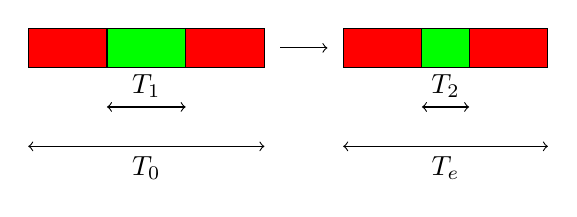
\begin{tikzpicture} [scale=1] %将图放大
\draw[fill=red] (-1,0) rectangle (0,0.5);
\draw[fill=green] (0,0) rectangle (1,0.5);
\draw[fill=red] (1,0) rectangle (2,0.5);
\draw[<->] (0, -0.5) -- (0.5, -0.5) node[above]{$T_1$} -- (1, -0.5);
\draw[<->] (-1, -1) -- (0.5, -1) node[below]{$T_0$} -- (2, -1);

\draw[->] (2.2,0.25) -- (2.8,0.25);
\draw[fill=red] (3,0) rectangle (4,0.5);
\draw[fill=green] (4,0) rectangle (4.6,0.5);
\draw[fill=red] (4.6,0) rectangle (5.6,0.5);
\draw[<->] (4, -0.5) -- (4.3, -0.5) node[above]{$T_2$} -- (4.6, -0.5);
\draw[<->] (3, -1) -- (4.3, -1) node[below]{$T_e$} -- (5.6, -1);
\end{tikzpicture}
\end{center}
$T_e=T_0[(1-f_e)+\frac{f_e}{S_e}]$, 其中$f_e=T_1/T_0$, $S_e=T_1/T_2$. 从而得到:
$$\mbox{系统加速比: }S=\frac{1}{(1-f_e)+f_e/S_e}$$
$$\mbox{多优化情况: }S=\frac{1}{(1-\sum f_e)+\sum\frac{f_e}{S_e}}$$

\section{指令系统}
\begin{itemize}
\item 四方面要求: 完备性, 有效性(存储空间小, 执行速度快, 访存效率+执行效率), 规整性(变长vs定长), 兼容性
\item 变长操作码设计例子: 最高四位是操作码, 但如果是1111, 就最高8位都是操作码, 类推.
	\begin{itemize}
	\item 例题: 指令字长16位, 操作数地址6位, 分0,1,2地址三种指令格式. 若采用扩展操作码技术, 二地址指令有X种, 零地址指令最多有Y种, 则一地址指令有几种?\\
	\ovalboxn{一条二地址指令可以换$2^6$条一地址指令(拿地址来编码),\\ 一条一地址指令也可以换$2^6$条零地址指令. \\设一地址指令有$M$条, 所以$Y=[(2^4-X)\times2^6-M]\times2^6$, \\进而$M=(2^4-X)\times2^6-Y\times2^{-6}$}
	\end{itemize}
\item MIPS的指令格式: I类, R类, J类. 有算逻, 控制, 访存指令.
	\begin{itemize}
	\item I类: 
		\begin{tabular}{|c|c|c|c|}
		\hline
	 	操作码(6) & rs(5) & rt(5) & 立即数(16) \\
		\hline
		\end{tabular}
		\begin{itemize}
		\item 立即寻址, 基址寻址, 相对寻址
		\end{itemize}
	\item R类: 
		\begin{tabular}{|c|c|c|c|c|c|}
		\hline
	 	操作码(6) & rs(5) & rt(5) & rd(5) & shamt(5, 位移量) & Funct(6) \\
		\hline
		\end{tabular}
		\begin{itemize}
		\item 寄存器寻址
		\end{itemize}
	\item J类: 
		\begin{tabular}{|c|c|}
		\hline
	 	操作码(6) & 与PC相加的偏移量(26) \\
		\hline
		\end{tabular}
		\begin{itemize}
		\item 伪直接寻址(26位形式地址左移两位与PC高4位拼接)
		\end{itemize}
	\end{itemize}

\end{itemize}

\section{MIPS处理器}
\subsection{单周期}
\subsection{多周期}
\begin{tabular}{|c|c|c|c|c|}
\hline
Step & R-Type & lw/sw & beq/bne & j	\\
\hline
IF & \multicolumn{4}{c|}{\begin{tabular}{c}IR=Mem[PC]\\PC=PC+4\end{tabular}} \\
\hline
ID & \multicolumn{4}{c|}{\begin{tabular}{c}A=Reg[IR[25-21]]\\B=Reg[IR[20-16]]\\ALUOut=PC+(SE(IR[15-0])<<2)\end{tabular}} \\
\hline
EX & ALUOut=A op B & ALUOut=A+SE(IR[15-0]) & \begin{tabular}{c}if(A==B)\\PC=ALUOut\end{tabular} & PC={PC[31:28],IR[25:0]$<<$2}\\
\hline
Mem & Reg[IR[15-11]]=ALUOut & \begin{tabular}{c}MDR=Mem[ALUOut]\\Mem[ALUOut]=B\end{tabular} & & \\
\hline
WB & & Reg[IR[20-16]]=MDR & & \\
\hline
\end{tabular}
\subsection{流水线}
\subsubsection{流水线分类}
\begin{itemize}
\item 单功能流水线/多功能流水线
\item 静态流水线: 同一时间只能有一个功能; 动态流水线: 同一时间可以有多功能
\item 指令流水线/宏流水线(多处理机)
\item 线性流水线/非线性流水线(有反馈)
\item 顺序流水线/乱序流水线
\end{itemize}
\subsubsection{流水线性能指标}
\begin{itemize}
\item 吞吐率: 取决于最慢的一段, 它是流水线的瓶颈(可以细分瓶颈, 或重复设置(第一个任务在第一段, 2在2, 3在1...))
	\begin{itemize}
	\item 各段相等均为$\Delta t_0$, 则$$TP_{max}=1/\Delta t_0$$
	\item 不等, 第$i$段为$\Delta t_i$, 则$$TP_{max}=1/max{\Delta t_i}$$
	\item 实际吞吐率: $TP=\frac{n}{T_{\mbox{流水}}}$, $T_{\mbox{流水}}=\sum\limits_{i=1}^m\Delta t_i+(n-1)\Delta t_j$(m为深度, n=任务数, $\Delta t_j$是最长的)
	\end{itemize}
\item 加速比: 流水线速度与非流水线速度之比(最大为段数m).$$S=T_{\mbox{非流水}}/T_{\mbox{流水}},\ T_{\mbox{非流水}}=nm\Delta t,\ T_{\mbox{流水}}=m\Delta t_0+(n-1)\Delta t_0$$
\item 效率: 部件运行时间/总时间, 也等于实际加速比/最大加速比m
\end{itemize}
\subsubsection{相关与冒险}
\begin{itemize}
\item 相关:
	\begin{itemize}
	\item 结构相关: 资源冲突. 解决方案: 流水线停顿, 哈佛结构等(访存结构化解)
	\item 数据相关: 需要用到前面指令的数据. 三类(写后读RAW(stall(软件叫nop)或旁路(转发Forward), 互锁(解决lw相关, lw后接需要EX的)), 写后写WAW(x), 读后写WAR(x))
	\item 控制相关: 分支或其他改变PC的指令时. 
		\begin{itemize}
		\item 延迟槽(delay slot): 跳转之后的无用功指令. 降低延迟开销的方法: 
			\begin{itemize}
			\item 提前beq到ID段(会有新的数据依赖问题, 甚至需要互锁)
			\item 延迟分支: 让某些必须做的指令放在延迟槽, 不管分支成不成功都应该执行; 可以从分支目标处调度, 从分支前指令调度, 从失败处调度, 找不到合适的指令就填nop.
			\item 分支预测技术: 静态预测(永远预测成功不成功, 往前往后成功不成功); 动态预测(一位饱和计数器, 两位饱和计数器)
			\end{itemize}
		\end{itemize}
	\end{itemize}
\end{itemize}
\subsubsection{流水线中的多发技术}
\begin{itemize}
\item 超标量技术: 配置多个功能部件, 以同时实现多个操作, 几乎每个单元都有两个. 一般是动态调度
\item 超长指令字技术: 可能长达几百位的指令, 将多条指令的功能拼到一起. 只有运算单元有两个. 一般是静态调度
\item 超流水线技术=深度流水线: 根据时钟上升下降沿各做一个, 主频不变, 但是变成两倍速度
\item SIMD技术: 数据拓宽, 寄存器变大.
\end{itemize}

\section{中断系统}
\subsection{中断异常的分类}
\begin{itemize}
\item x86: 外部中断(可屏蔽/不可屏蔽中断), 内部中断(软中断, 系统调用INT, 指令断点(调试))
\item RISC: 包含外部事件, 异常, 陷阱
\end{itemize}
\subsection{中断异常发生的时机}
\begin{itemize}
\item I/O中断Interrupts(随时发生, 当前指令完才响应)
\item 异常Exception(随时发生, 随时处理)
\item 陷阱Traps(专用指令, 特殊处理)(主要在OS涉及)
\end{itemize}
\subsection{中断主要内容}
\subsubsection{中断机构}
\begin{itemize}
\item PSW程序状态字: 有中断标志位
\item 一个中断源对应一个INTR中断请求标记触发器
\end{itemize}
\subsubsection{中断判优}
\begin{itemize}
\item 软件中程序查询
\item 硬件排队器: 可以集中在CPU内或分散在中断源接口电路.
\end{itemize}
\subsubsection{中断响应}
\begin{itemize}
\item 中断隐指令: 保护程序断电, 寻找服务程序入口(硬件向量法(多一条jmp指令), 中断程序入口), 可能需要关中断
\end{itemize}
\subsubsection{保护和恢复现场}
\begin{itemize}
\item 保护现场包括断点(中断隐指令完成), 寄存器内容(中断服务程序完成)
\item 恢复现场, 然后返回.
\end{itemize}
\subsubsection{中断屏蔽技术——实现了动态优先级}
\begin{itemize}
\item 在排队器加mask之类的
\item 可以修改优先级置屏蔽字, 在保护现场和开中断之间去设置屏蔽字(这样开了中断屏蔽字才是对的), 在恢复现场和开中断之间恢复屏蔽字
\item 响应优先级(不改变), 处理优先级(可改变, 通过置屏蔽字)
\end{itemize}
\subsubsection{硬件代价}
\begin{itemize}
\item EPC寄存器保存异常指令的地址
\item 状态寄存器cause
\end{itemize}
\subsection{流水线的异常处理}
\begin{itemize}
\item 非精确处理: 允许进入流水线的指令执行完再处理中断, 只要发生异常不论在哪段, 后续指令都不让进去. 需要操作系统来支持, 硬件很简单. 简称甩锅hhh; 另一种方法是视异常位控制相关. 后续指令排空. 异常响应时间长, 可能导致程序出错, 调试不便.
\item 精确处理: 提交点技术实现.
	\begin{itemize}
	\item 多个异常: 先发生的异常不立即处理, 只是标记, 最深的指令优先(早期异常抑制后面的).
	\item 放在Mem段是保证前面的指令都处理完了, 后续指令还没有写回, 并尽可能收集了错误.
	\end{itemize}
	
\end{itemize}

\section{存储器}
\subsection{主存简介}
\begin{itemize}
\item 技术指标: 存储容量, 存取时间, 存储周期(连续两次存取需要的间隔时间), 存储器带宽
\item 芯片结构: 译码驱动, 读写电路, 控制线(读写控制线, 片选线)
\item SRAM随机存储器(锁存器, 重合法译码(行列选))都是易失性存储. 主要用于缓存, 因为快.
	\begin{itemize}
	\item 读写周期: 读出时间(放上有效地址到数据有效), 读周期时间(放地址到读完); 写入时间(写的时间), 维持时间(写完要维持的时间), 写周期时间(整个); 存取周期(读周期=写周期)
	\end{itemize}
\item DRAM: 电容, 先放行, 再放列, 都有锁存器, 按行刷新(集中刷新(有时间间隔), 分散刷新(穿插读写之中))
\item 只读存储器ROM
\item 位扩展: 横向容量, 地址线控制线公用, 数据线分开
\item 字扩展: 纵向容量, 数据线和地址线公用, 读写控制线公用, 片选使能分开
\item CPU地址线一般比存储芯片多, 低位线连接存储芯片地址线, 高位连接片选
\item 提高访存速度: 双端口存储器, 高速主存, 并行访问存储器, 层次化存储结构
	\begin{itemize}
	\item 并行存储手段: 单体多字(一次缓存多字, 局部性原理), 多体并行(预取, 流水传输)
		\begin{itemize}
		\item 高位交叉: 地址0到n-1都在$M_0$, n到2n-1都在$M_1$, 也就是高位表示选片. 方便扩容, 支持并行访问
		\item 低位交叉: 并行访问, 提高带宽
		\end{itemize}
	\end{itemize}
\item 容错与校验: 信息冗余(海明码, CRC码, 奇偶校验码), 时间冗余(回滚), 空间冗余(复用, 磁盘冗余阵列)
	\begin{itemize}
	\item 码距: 任意两个编码的最小海明距离. 为了检测D个误码, 需要最小码距$L\ge D+1$; 为了纠正C个误码, 需要最小码距$L\ge 2C+1$. $L-1\ge C+D$且$D\ge C$
	\item 奇偶校验: 加一位校验位. 奇校验(1个数为奇数), 偶校验(1个数为偶数). $L-1\ge C+D$, $D\ge C$, 所以$C=0, D=1$
	\item 海明码(Hamming): $2^r-1\ge r+k$, r是数据位数, k是校验码位数
	\item CRC循环冗余校验
	\end{itemize}
\end{itemize}
\subsection{高速缓冲存储器Cache}
\begin{itemize}
\item 解决速度不匹配, 解决设备冲突
\item Cache和主存交换单位为块
\item 命中率(h), 平均访存时间, 效率(=全命中时间/访存时间), 容量越大命中率越高(有极限), 随着块长增高, 命中率先+后-
\item Cache和主存的地址映射
	\begin{itemize}
	\item 全相联映射: 主存的每一块都可以映射到Cache里任意位置. 主存地址=s+w位. 需要高速相联存储器
	\item 直接映射: Cache块号=主存块号 mod m(Cache块数), 因此只需要一次比较(比较可能在的唯一那一Cache块)
	\item 组相联映射: 放在哪个组固定, 但组内哪块不固定. Cache块数=组数u*块数v. 称为v路组相联
	\end{itemize}
\item 一致性问题: 写策略(写直达法, 写回法, 及是否按写分配(写未命中是否调块))
\end{itemize}
\subsection{虚存}
\begin{itemize}
\item 页表基址寄存器
\item TLB快表
\end{itemize}

\section{总线}
\subsection{总线概述}
\subsection{总线结构}
\begin{itemize}
\item 单总线结构: 全都挂在一个总线上. 把CPU和IO放一起, 速度不匹配, 而且容易冲突; 易扩展.
\item 双总线: CPU, 主存为一个, IO等为另一个, 中间由通道连接
\item 三总线: 在双总线上, CPU和IO到内存都由单独的总线
\item ...
\end{itemize}
\subsection{总线仲裁(总线判优)}
\begin{itemize}
\item 集中式仲裁: 集中在CPU, 每个模块有总线请求信号线BR和总线授权信号线BG; 
	\begin{itemize}
	\item 链式查询: 优先级为离仲裁器近的高, 硬件简单, 会造成饥饿
	\item 计数器定时查询: 接到请求就开始计数, 设备比较一样就得到总线
	\item 独立请求: 每个设备有一对请求授权线
	\end{itemize}
\item 分布式仲裁
	\begin{itemize}
	\item 自举分布式仲裁: 独立判断自己是否是最高优先级请求者
	\item 冲突检测分布式仲裁: 冲突时会被检测到
	\item 并行竞争分布式仲裁: 
	\end{itemize}
\end{itemize}
\subsection{总线通信}
\begin{itemize}
\item 总线操作: 读写操作, 块传送操作(猝发式操作(Burst)), 写后读(校验), 广播广集
\item 总线周期: 申请分配阶段, 寻址阶段, 传送阶段, 结束阶段
\item 传输方式: 串行/并行, 分时复用(既传数据又传地址等)
\item 同步通信: 通信双方时钟统一, 通常由CPU给出, 也可以用全局时钟
\item 异步通信: 没有公共时钟标准. 采用应答, 握手方式. 有不互锁(请求发过去就好了), 半互锁(发请求, 等应答回来再去做), 全互锁(请求, 应答, 确认收到)
\item 比特率: 有效数据(bps); 波特率: 所有数据(bps)
\item 半同步通信: 地址命令数据都是按照时钟沿发的, 但有等待信号线(等他就绪了再来取数据), 用于要等不确定时间或很久的情况.
\item 总线传输周期: 发出地址命令开始到数据传输结束
\item 分离式通信: 主设备获得总线后发地址和命令, 然后放弃, 等模块准备好了, 再申请总线使用权, 和相应设备通信
\end{itemize}

\section{I/O系统}
\subsection{I/O系统的组成}
\begin{itemize}
\item I/O指令, 通道指令
\item 统一编址: I/O设备看作存储器的一部分; 独立编制: 需要专门的IO指令
\item 并行传送/串行传送
\item 立即响应/异步应答/同步联络
\end{itemize}
\subsection{I/O接口}
\begin{itemize}
\item 两个设备之间的连接电路及其对应软件控制
\item 为什么需要接口: 
	\begin{itemize}
	\item 设备选择
	\item 缓冲
	\item 串并转换, 电平转换
	\item 传送控制命令
	\item 监视设备工作状态
	\end{itemize}
\item 端口: 接口电路中的一些寄存器
\end{itemize}
\subsection{信息交换方式}
\begin{itemize}
\item 程序查询方式: 通过IO指令查询忙之类的状态, 硬件上需要数据线地址线命令线等等.
\item 程序中断方式: 外设发出中断
\item DMA方式: 完全由硬件执行IO交换, 只有控制信号逻辑通过CPU做. 传送前后要通过程序或中断方式对缓冲器和DMA控制器作相关操作. 避免CPU和DMA访存冲突的方法(DMA工作时CPU不能访存, 周期挪用/窃取(CPU访存时, DMA窃取一个或多个周期来访存), 交替访存); 有公用DMA请求和独立DMA请求(区别在多个DMA是否用同一条线)
\item 通道方式: 一个主机多个通道, 每个通道多个IO设备. 
\end{itemize}




\newpage
\keypoint{Booth算法}{https://www.cnblogs.com/raymon-tec/p/5014229.html}

\end{document}






